\documentclass[tikz,border=6pt]{standalone}
\usepackage{amsmath}
\usetikzlibrary{arrows.meta}
\begin{document}
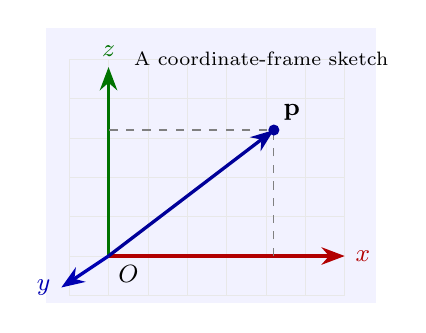
\begin{tikzpicture}[
  >=Stealth,
  axis/.style={very thick,->},
  every node/.style={font=\small}
]
  \fill[blue!5] (-0.8,-0.6) rectangle (3.4,2.9);
  \draw[step=0.5,gray!18,very thin] (-0.5,-0.5) grid (3,2.5);
  \draw[axis,red!70!black] (0,0) -- (3,0) node[right] {$x$};
  \draw[axis,green!45!black] (0,0) -- (0,2.4) node[above] {$z$};
  \draw[axis,blue!70!black] (0,0) -- (-0.6,-0.4) node[left] {$y$};
  \draw[dashed,gray] (2.1,0) -- (2.1,1.6) -- (0,1.6);
  \draw[very thick,->,blue!60!black] (0,0) -- (2.1,1.6);
  \fill[blue!60!black] (2.1,1.6) circle (2pt);
  \node[above right] at (2.1,1.6) {$\mathbf{p}$};
  \node[below right] at (0,0) {$O$};
  \node[anchor=west,font=\scriptsize] at (0.2,2.5) {A coordinate-frame sketch};
\end{tikzpicture}
\end{document}
